\section{Parallélisation du code (MPI) --- Première façon}

\subsection{Stratégie de parallélisation}

\subsubsection{Objectif}

L'objectif de cette étape est de réduire le temps noyau \(K0\) via une exécution distribuée
(MPI), puis de mesurer l'accélération en fonction du nombre de processus.
On conserve la même logique expérimentale que pour OpenMP : mode benchmark, no-render,
plusieurs répétitions, et calcul du speedup.

\subsubsection{Choix d'architecture}

Dans notre implémentation \texttt{mpi1}, on ajoute un backend dédié \texttt{mpi1+soa}
(sélectionné via \texttt{--exec mpi1 --layout soa}).
Les modes existants \texttt{serial} et \texttt{omp} sont conservés tels quels
(même comportement, même logique de benchmark). Le code MPI est ainsi isolé dans un chemin
d'exécution spécifique, afin d'éviter toute régression sur les autres modes.

\subsubsection{Répartition du travail}

Le principe de la ``première façon'' est :
\begin{itemize}[leftmargin=*]
  \item chaque processus MPI possède une copie complète de l'environnement
  (terrain, obstacles, phéromones \(V1/V2\), nid, nourriture) ;
  \item les fourmis sont réparties par indices (bloc par rang \texttt{rank}) ;
  \item chaque rang simule uniquement sa plage locale de fourmis.
\end{itemize}

Ce choix est simple à implémenter et ne requiert pas de migration de fourmis entre rangs.

\subsubsection{Communications et synchronisation}

Dans \texttt{mpi1}, on conserve :
\begin{itemize}[leftmargin=*]
  \item \texttt{MPI\_Allreduce(..., MPI\_MAX)} pour fusionner les cartes \(V1/V2\) ;
  \item \texttt{MPI\_Allreduce(..., MPI\_SUM)} pour agréger le \texttt{food\_delta} (quantité de nourriture collectée)
  et maintenir une métrique globale cohérente.
\end{itemize}

\paragraph{Contrôle de granularité.}
La version actuelle ajoute un paramètre de granularité :
\begin{itemize}[leftmargin=*]
  \item \texttt{--mpi-sync-every K} (par défaut \(K=1\)) ;
  \item la fusion \(V1/V2\) est effectuée une fois toutes les \(K\) itérations.
\end{itemize}
Le compteur de nourriture reste synchronisé \emph{à chaque itération} (payload faible),
et la sortie benchmark est imprimée uniquement par le rang 0 (root-only), afin de préserver
un format \texttt{METRIC ...} propre et facilement parsable.

\subsubsection{Correctness et cohérence}

MPI travaille en mémoire distribuée : chaque rang a son propre espace mémoire.
On évite donc les data races de type mémoire partagée entre processus.
La cohérence globale est assurée par les collectives :
\begin{itemize}[leftmargin=*]
  \item \texttt{MAX} pour la fusion des phéromones, cohérent avec un ordre de traitement
  potentiellement arbitraire des fourmis entre rangs ;
  \item \texttt{SUM} pour maintenir un compteur global de nourriture cohérent.
\end{itemize}

\subsubsection{Profilage et métriques MPI}

En MPI, le temps global d'une itération correspond au temps du rang le plus lent.
Pour chaque métrique temporelle (\(K0\), \(K1\), \(K4\), \(K5\), et \(K_{\text{MPI\_sync}}\)),
on retient donc :
\[
T_p = \max_{r \in \{0,\dots,p-1\}} T_p^{(r)}
\]
via \texttt{MPI\_Allreduce(..., MPI\_MAX)} sur les temps locaux.
Ce choix correspond aussi à l'idée de \emph{load balancing} : le temps parallèle est pénalisé
par le processus le plus lent, et toute variabilité (bruit système, déséquilibre) se répercute
sur le temps global.

On introduit \(K_{\text{MPI\_sync}}\) pour isoler le coût des synchronisations collectives
(\texttt{Allreduce}) et interpréter la scalabilité.

\subsection{Résultat du Profilage}

\subsubsection{Protocole expérimental}

Campagne utilisée dans cette section :
\begin{itemize}[leftmargin=*]
  \item \texttt{results/test\_mpi1\_sync\_every\_rerun/20260307\_155513}
\end{itemize}

Commande type :
\begin{verbatim}
OMP_NUM_THREADS=1 OMP_DYNAMIC=FALSE \
mpirun --bind-to core --map-by core -np P ./src/ant_simu.exe \
  --exec mpi1 --layout soa --benchmark --no-render \
  --iterations 400 --warmup 100 --mpi-sync-every K
\end{verbatim}

Balayages réalisés :
\[
P \in \{1,2,4,8\}, \qquad K \in \{1,5,10\}
\]
avec \textbf{1 coeur par processus}.

Paramètres de campagne :
\begin{itemize}[leftmargin=*]
  \item répétitions : \texttt{reps = 3} ;
  \item warmup : \texttt{100} itérations ;
  \item itérations mesurées : \texttt{300} (sur 400 totales) ;
  \item machine : AMD Ryzen 7 5800H, WSL2, Open MPI 4.1.6.
\end{itemize}

Le speedup est calculé à \(P=1\) \textbf{pour chaque valeur de \(K\)} :
\[
S_K(p)=\frac{T_K(1)}{T_K(p)}, \qquad E_K(p)=\frac{S_K(p)}{p}
\]

\paragraph{Remarque sur la mesure du speedup.}
Le cours rappelle que l'algorithme séquentiel peut différer de l'algorithme parallèle
(et que la mesure du speedup n'est alors pas ``évidente'').
Ici, nous prenons comme référence \textbf{MPI1 à \(P=1\)} (pour une valeur donnée de \(K\)),
afin de comparer un \emph{même algorithme} et d'isoler l'effet du parallélisme MPI.
La comparaison avec \texttt{serial+soa} reste utile comme contrôle, mais n'est pas utilisée
comme référence principale du speedup MPI1.

\subsubsection{Scénario de scalabilité (cours)}

Nous évaluons ici le \emph{worst speedup} : la quantité de données \emph{globale} est fixée
(nombre total de fourmis, taille de la carte) et on augmente uniquement le nombre de processus \(P\).
Dans un scénario \emph{best speedup}, on conserverait une quantité de données fixe \emph{par processus}
(en augmentant par exemple le nombre total de fourmis avec \(P\)), ce qui tend à améliorer
le speedup.

\subsubsection{Baseline MPI1 (\(K=1\), sync à chaque itération)}

La variation relative du temps noyau est définie par :
\[
\Delta(K0_p)=K0_p-K0_1,
\qquad
\Delta_{\%}(K0_p)=100\times\frac{K0_p-K0_1}{K0_1}
\]
où \(K0_1\) désigne la valeur mesurée avec 1 processus.

\begin{table}[H]
\centering
\scriptsize
\caption{MPI1 SoA (\(K=1\)) : temps noyau, variation relative et speedup selon le nombre de processus}
\label{tab:mpi1-speedup-k1}
\begin{tabular}{@{}rrrrrrr@{}}
\toprule
\textbf{np} & \textbf{K0 moyen} & \textbf{écart-type} & \textbf{\(\Delta\)} & \textbf{\(\Delta_{\%}\)} & \textbf{Speedup \(S(p)\)} & \textbf{Efficacité \(E(p)\)} \\
\midrule
1 & 6.632929 & 0.069502 & +0.000000 & +0.000 & 1.000000 & 1.000000 \\
2 & 5.875666 & 0.309316 & -0.757263 & -11.417 & 1.128881 & 0.564441 \\
4 & 9.602010 & 0.587313 & +2.969081 & +44.763 & 0.690786 & 0.172696 \\
8 & 19.178292 & 0.892592 & +12.545363 & +189.138 & 0.345856 & 0.043232 \\
\bottomrule
\end{tabular}
\end{table}

\[
S_{\text{th,idéal}}(p)=p
\]

\begin{table}[H]
\centering
\caption{Comparaison speedup mesuré vs speedup théorique idéal (MPI1 SoA, \(K=1\))}
\label{tab:mpi1-speedup-theory-k1}
\begin{tabular}{@{}rrrr@{}}
\toprule
\textbf{np} & \textbf{\(S_{\text{mesuré}}(p)\)} & \textbf{\(S_{\text{th,idéal}}(p)\)} & \textbf{\(S_{\text{mesuré}}/S_{\text{th,idéal}}\)} \\
\midrule
1 & 1.000000 & 1.000000 & 1.000000 \\
2 & 1.128881 & 2.000000 & 0.564441 \\
4 & 0.690786 & 4.000000 & 0.172696 \\
8 & 0.345856 & 8.000000 & 0.043232 \\
\bottomrule
\end{tabular}
\end{table}

La table met en évidence l'écart au modèle idéal: à \(np=8\), MPI1 n'atteint que
\(4.3\%\) du speedup linéaire théorique. Cette lecture est cohérente avec la domination
de \(K_{\text{MPI\_sync}}\) observée dans la décomposition des kernels.

\begin{table}[H]
\centering
\caption{Décomposition du noyau MPI1 SoA (\(K=1\))}
\label{tab:mpi1-breakdown-k1}
\begin{tabular}{@{}rrrrr@{}}
\toprule
\textbf{np} & \textbf{K1 (ms/iter)} & \textbf{K4 (ms/iter)} & \textbf{K5 (ms/iter)} & \(\mathbf{K_{\text{MPI\_sync}}}\) \textbf{(ms/iter)} \\
\midrule
1 & 6.304193 & 0.312222 & 0.007008 & 0.006936 \\
2 & 3.709763 & 0.694195 & 0.013545 & 1.571793 \\
4 & 2.523657 & 1.906690 & 0.040042 & 5.304413 \\
8 & 1.647622 & 4.160358 & 0.101536 & 13.420741 \\
\bottomrule
\end{tabular}
\end{table}

\begin{figure}[H]
  \centering
  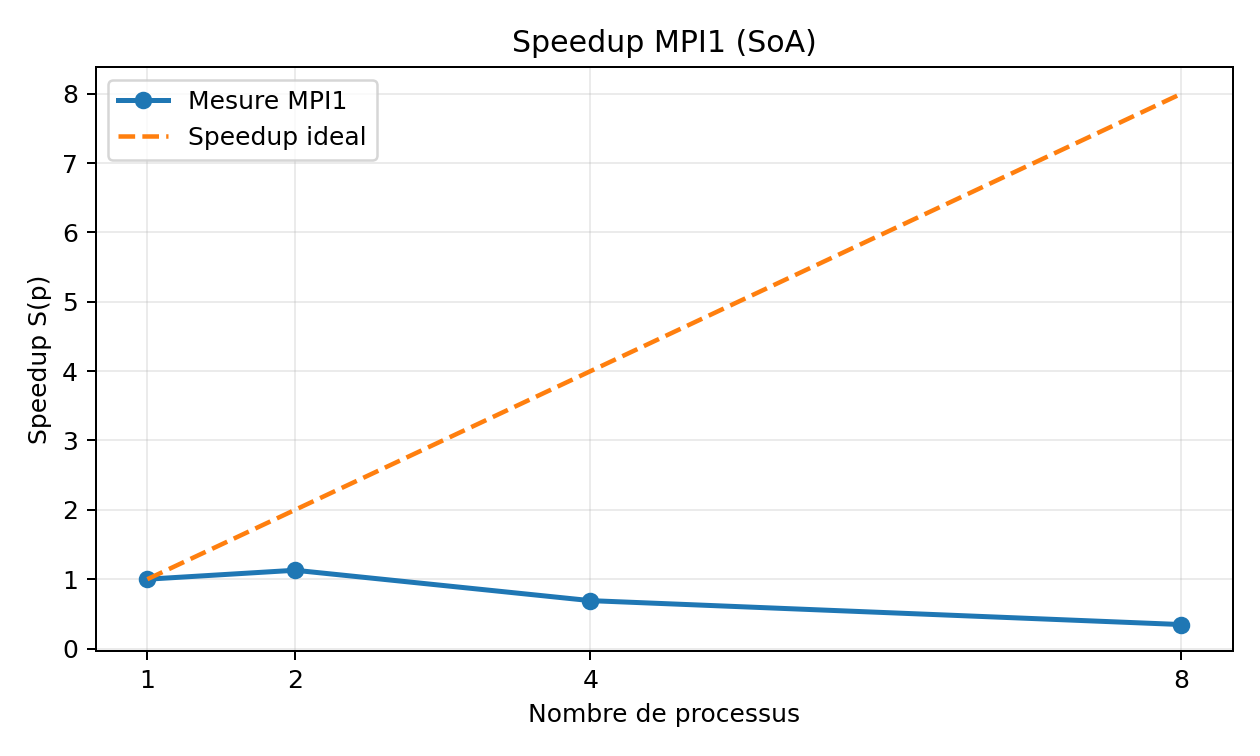
\includegraphics[width=0.82\textwidth]{imgs/mpi1/mpi1_speedup.png}
  \caption{Speedup mesuré MPI1 (SoA) pour \(K=1\) vs speedup idéal linéaire}
  \label{fig:mpi1-speedup}
\end{figure}

\subsubsection{Définition et lecture de l'efficacité}

L'efficacité est définie par :
\[
E(p)=\frac{S(p)}{p}
\]

Une efficacité proche de 1 signifie que les processus supplémentaires sont utilisés de manière
efficace. Lorsqu'elle diminue, cela indique qu'une part croissante du temps est perdue dans les
overheads de parallélisation. En MPI1, cette baisse d'efficacité vient surtout du coût des
synchronisations globales et des communications collectives sur les cartes complètes \(V1/V2\).

\begin{figure}[H]
  \centering
  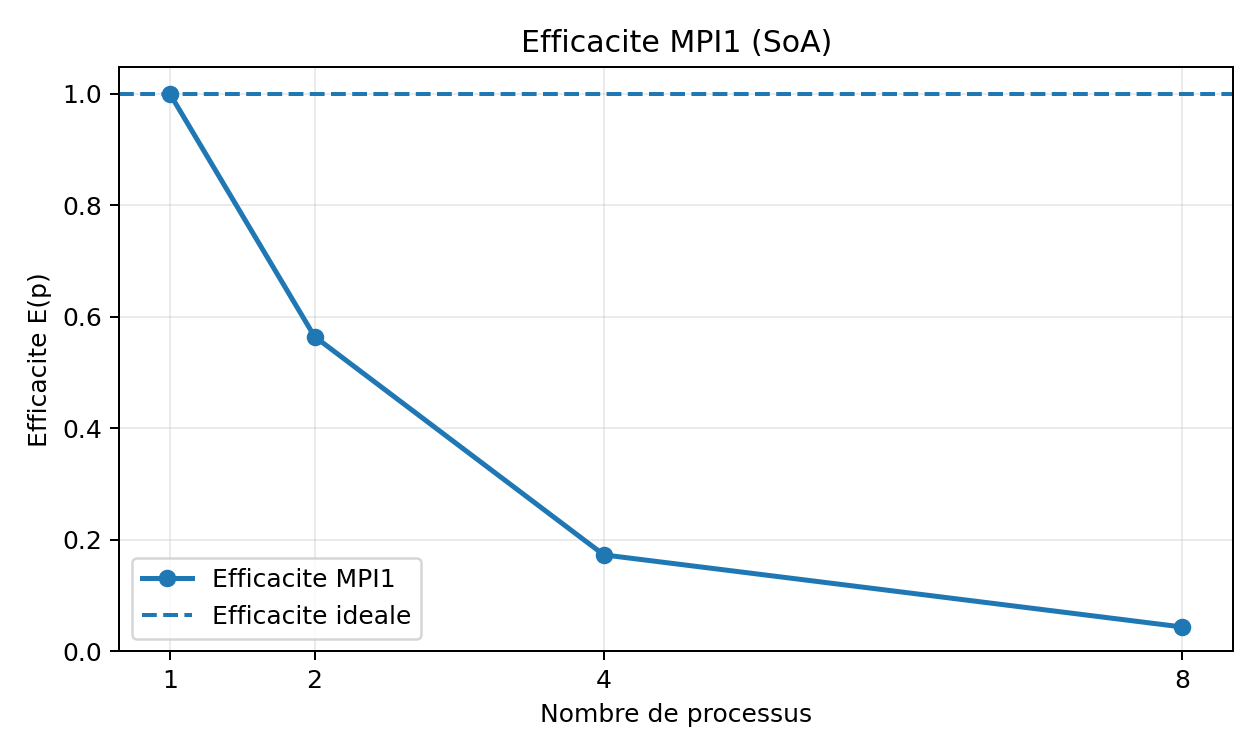
\includegraphics[width=0.82\textwidth]{imgs/mpi1/mpi1_efficiency.png}
  \caption{Efficacité MPI1 (SoA) en fonction du nombre de processus}
  \label{fig:mpi1-efficiency}
\end{figure}

\begin{figure}[H]
  \centering
  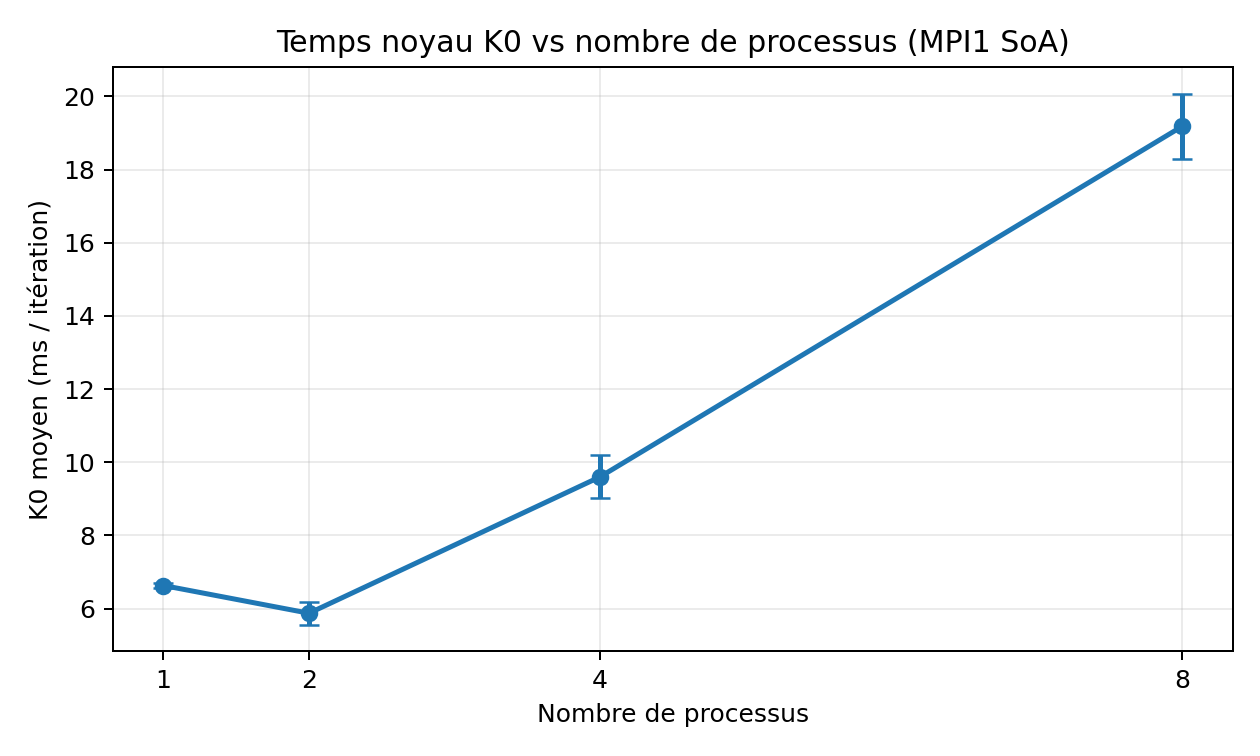
\includegraphics[width=0.82\textwidth]{imgs/mpi1/mpi1_k0_ms_iter.png}
  \caption{Temps noyau \(K0\) en fonction du nombre de processus (\(K=1\))}
  \label{fig:mpi1-k0}
\end{figure}

\begin{figure}[H]
  \centering
  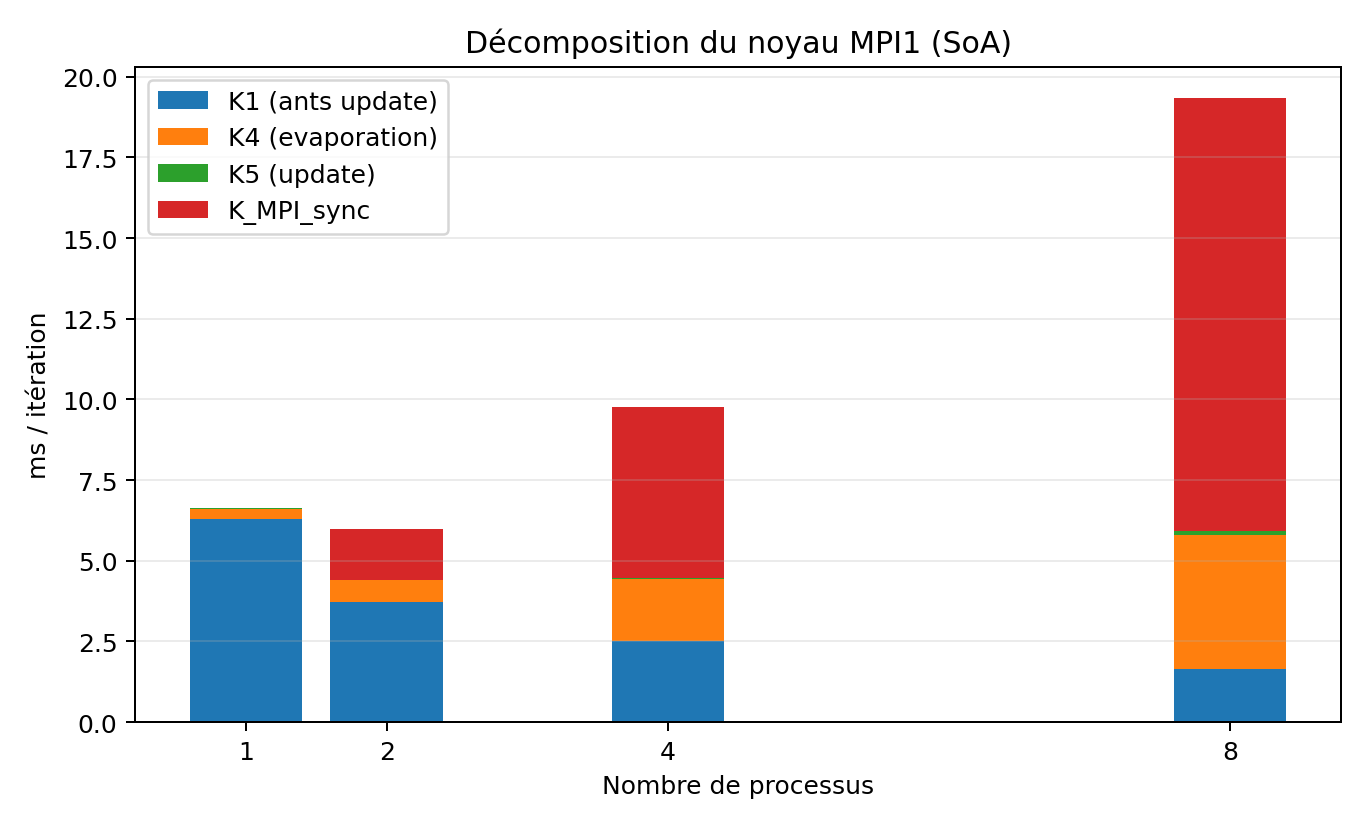
\includegraphics[width=0.84\textwidth]{imgs/mpi1/mpi1_kernel_breakdown.png}
  \caption{Décomposition \(K1/K4/K5/K_{\text{MPI\_sync}}\) du noyau MPI1 SoA (\(K=1\))}
  \label{fig:mpi1-breakdown}
\end{figure}

\subsubsection{Impact de \texttt{mpi\_sync\_every}}

\begin{table}[H]
\centering
\caption{Impact de la fréquence de synchronisation sur la scalabilité MPI1}
\label{tab:mpi1-sync-every-impact}
\begin{tabular}{@{}rrrrr@{}}
\toprule
\textbf{K} & \textbf{\(S_K(2)\)} & \textbf{\(S_K(4)\)} & \textbf{\(S_K(8)\)} & \textbf{Part \(K_{\text{MPI\_sync}}\) à \(np=8\)} \\
\midrule
1  & 1.128881 & 0.690786 & 0.345856 & 69.98\% \\
5  & 1.440629 & 1.228152 & 0.695220 & 33.02\% \\
10 & 1.467855 & 1.385889 & 0.763005 & 22.74\% \\
\bottomrule
\end{tabular}
\end{table}

\begin{figure}[H]
  \centering
  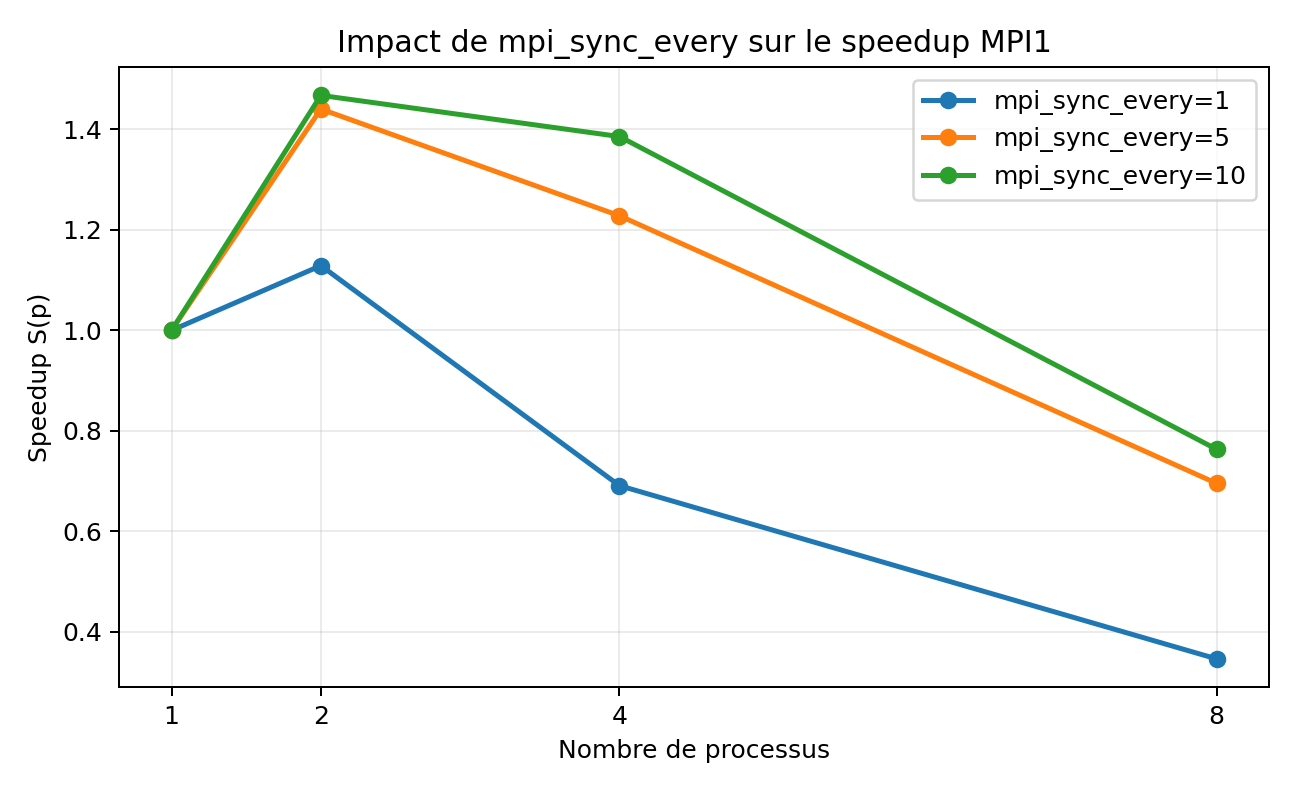
\includegraphics[width=0.82\textwidth]{imgs/mpi1/mpi1_sync_every_speedup.png}
  \caption{Effet de \texttt{mpi\_sync\_every} sur le speedup MPI1}
  \label{fig:mpi1-sync-every-speedup}
\end{figure}

\begin{figure}[H]
  \centering
  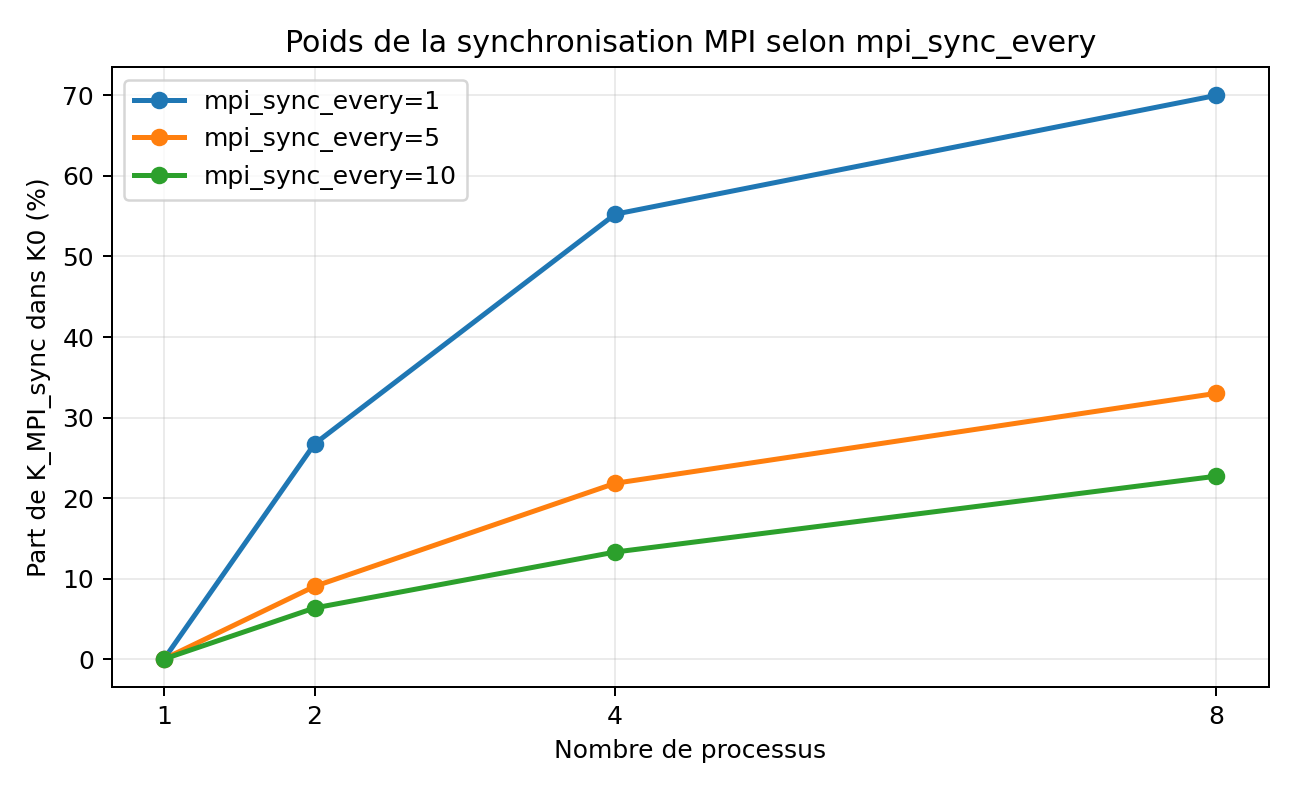
\includegraphics[width=0.82\textwidth]{imgs/mpi1/mpi1_sync_every_kmpi_share.png}
  \caption{Part de \(K_{\text{MPI\_sync}}\) dans \(K0\) selon \texttt{mpi\_sync\_every}}
  \label{fig:mpi1-sync-every-share}
\end{figure}

\subsection{Analyse des Résultats}

\subsubsection{Comportement global et scalabilité}

Avec la baseline \(K=1\), on observe :
\begin{itemize}[leftmargin=*]
  \item un petit gain à \(np=2\) (\(S(2)=1.13\)) ;
  \item une dégradation nette ensuite (\(S(4)=0.69\), \(S(8)=0.35\)).
\end{itemize}

La Table~\ref{tab:mpi1-speedup-theory-k1} confirme que l'écart au speedup idéal se creuse
très rapidement avec \(np\): le comportement passe d'un gain modeste à \(np=2\) à une
régression marquée dès \(np=4\), ce qui est typique d'un régime dominé par la communication.

\subsubsection{Lecture ``granularité'' et coût de communication}

Le cours rappelle qu'un échange de messages comporte (i) un coût initial (constant) et
(ii) un coût de transfert proportionnel à la quantité de données.
Dans MPI1, la fusion des phéromones utilise des collectives \texttt{Allreduce(MAX)} sur les
\textbf{cartes complètes} \(V1/V2\), ce qui implique un volume de données élevé à chaque synchronisation.
Ainsi, lorsque \(np\) augmente, le coût de communication et de synchronisation peut dominer le temps total,
ce qui limite (voire inverse) le speedup.

La cause principale est bien \(K_{\text{MPI\_sync}}\), qui devient dominant quand \(np\) augmente :
sa part passe d'environ \(0.10\%\) à \(np=1\) à \(69.98\%\) à \(np=8\).
Dans cette ``première façon'', on échange les cartes complètes \(V1/V2\) ; le coût de synchronisation
croît donc rapidement avec le nombre de processus.

\subsubsection{Lecture de l'efficacité}

La Figure~\ref{fig:mpi1-efficiency} et la Table~\ref{tab:mpi1-speedup-k1} montrent que l'efficacité
chute très vite avec \(np\) dans la baseline \(K=1\) (\(E(2)=0.5644\), \(E(4)=0.1727\), \(E(8)=0.0432\)).
Cette baisse est cohérente avec la domination progressive de \(K_{\text{MPI\_sync}}\).
Autrement dit, même si le calcul local sur les fourmis est mieux réparti, le coût des synchronisations
globales absorbe une part de plus en plus grande du gain potentiel. Les essais avec \(K>1\) améliorent
partiellement cette efficacité, ce qui confirme que le principal verrou est bien la communication.

\subsubsection{Pourquoi \(K4\) augmente avec \(np\) (régime memory-bound)}

Même si MPI est un modèle ``mémoire distribuée'', nos expériences sont réalisées sur une seule machine.
Quand \(np\) augmente, plusieurs processus balaient la carte de phéromones en même temps, ce qui
peut saturer la bande passante mémoire et dégrader \(K4\) (régime \emph{memory-bound}).
Ce comportement est cohérent avec les limites liées aux accès mémoire : un balayage de grille
parallélise le calcul, mais peut rester limité par la mémoire.

\subsubsection{Effet de \texttt{mpi\_sync\_every} (trade-off cohérence / performance)}

L'ajout de \texttt{--mpi-sync-every K} confirme l'analyse ``granularité vs communication'' :
\begin{itemize}[leftmargin=*]
  \item en réduisant la fréquence des \texttt{Allreduce(MAX)}, la part de \(K_{\text{MPI\_sync}}\)
  diminue fortement (à \(np=8\) : 69.98\% \(\rightarrow\) 33.02\% \(\rightarrow\) 22.74\% pour
  \(K=1,5,10\)) ;
  \item la scalabilité s'améliore sensiblement (\(S_5(4)=1.23\), \(S_{10}(4)=1.39\)) ;
  \item à \(np=8\), le speedup reste inférieur à 1 sur cette machine, mais la régression est nettement
  réduite (\(0.35 \rightarrow 0.70 \rightarrow 0.76\)).
\end{itemize}

En termes simples, \texttt{mpi\_sync\_every} augmente la granularité en réduisant le nombre
d'échanges globaux : moins de synchronisations \(\Rightarrow\) moins de coût de communication par itération.
En contrepartie, la cohérence globale des cartes \(V1/V2\) est moins fréquente (une fois toutes les \(K\) itérations),
ce qui correspond à un compromis performance / cohérence.

\subsubsection{Remarque sur le temps MPI (wall-time)}

Le temps rapporté est un \emph{wall-time} MPI (maximum entre rangs).
Toute variabilité (déséquilibre léger, bruit système WSL2) est donc payée globalement,
ce qui peut amplifier \(K0\) lorsque \(np\) augmente.

\subsection{Interprétation}

Les résultats des Tables~\ref{tab:mpi1-speedup-k1}, \ref{tab:mpi1-breakdown-k1} et
\ref{tab:mpi1-sync-every-impact}, ainsi que des Figures~\ref{fig:mpi1-speedup},
\ref{fig:mpi1-efficiency}, \ref{fig:mpi1-breakdown}, \ref{fig:mpi1-sync-every-speedup} et
\ref{fig:mpi1-sync-every-share}, conduisent à une conclusion assez nette.

La ``première façon'' MPI fonctionne correctement du point de vue algorithmique:
la répartition des fourmis par rang est bien opérationnelle, la cohérence globale des cartes
de phéromones est maintenue par \texttt{Allreduce(MAX)}, et les temps sont interprétés
correctement comme des \emph{wall-times} MPI via un maximum entre rangs.
Autrement dit, l'implémentation est valide comme baseline distribuée.

En revanche, les résultats montrent aussi que cette stratégie scale mal lorsque le nombre de
processus augmente. La Table~\ref{tab:mpi1-speedup-k1} et la Figure~\ref{fig:mpi1-speedup}
montrent qu'avec une synchronisation à chaque itération (\(K=1\)), le gain est très limité à
\(np=2\), puis devient une régression à \(np=4\) et \(np=8\).
La Table~\ref{tab:mpi1-breakdown-k1} et la Figure~\ref{fig:mpi1-breakdown} expliquent pourquoi:
\(K_{\text{MPI\_sync}}\) devient progressivement la composante dominante du coût total.

Le paramètre \texttt{mpi\_sync\_every} confirme directement l'interprétation issue du cours sur
la granularité. Lorsque l'on réduit la fréquence des synchronisations globales, le poids de
\(K_{\text{MPI\_sync}}\) diminue fortement et le speedup s'améliore nettement, comme on le voit
dans la Table~\ref{tab:mpi1-sync-every-impact} et les Figures~\ref{fig:mpi1-sync-every-speedup}
et \ref{fig:mpi1-sync-every-share}. Cela montre que, dans notre cas, la limite principale n'est
pas le calcul local sur les fourmis, mais bien le coût des communications collectives sur les
cartes globales \(V1/V2\).

La lecture finale est donc la suivante: MPI1 constitue une première version cohérente et simple à
analyser, mais son coût de synchronisation globale devient trop élevé dès que \(np\) augmente.
Cette campagne justifie donc naturellement la transition vers la ``deuxième façon'' du projet,
c'est-à-dire une décomposition de domaine avec échanges plus locaux, afin de réduire le volume
de communication globale par itération.
